\section{Discussion and Evaluation}
\label{sec:discussion}
We evaluate the impact on the consumption trace for our system in figure \ref{CompPlots} and \ref{interactiveLoads}. In figure \ref{interactiveLoads} the consumption trace of all interactive loads is displayed. The consumption varies throughout the day with various peaks, typically at 30 to 60 watts. However, there is one very large peak around 14:00 at approximately 230 watts. It will not be possible for our system to counteract the highest peak since we cannot control the interactive loads. Therefore, the best achievable maximum peak cannot be below the 230 watts from the interactive loads. It will furthermore not be possible for our scheduler to know about this peak beforehand and it cannot make decisions thereafter.

\begin{figure}[!ht]
\centering
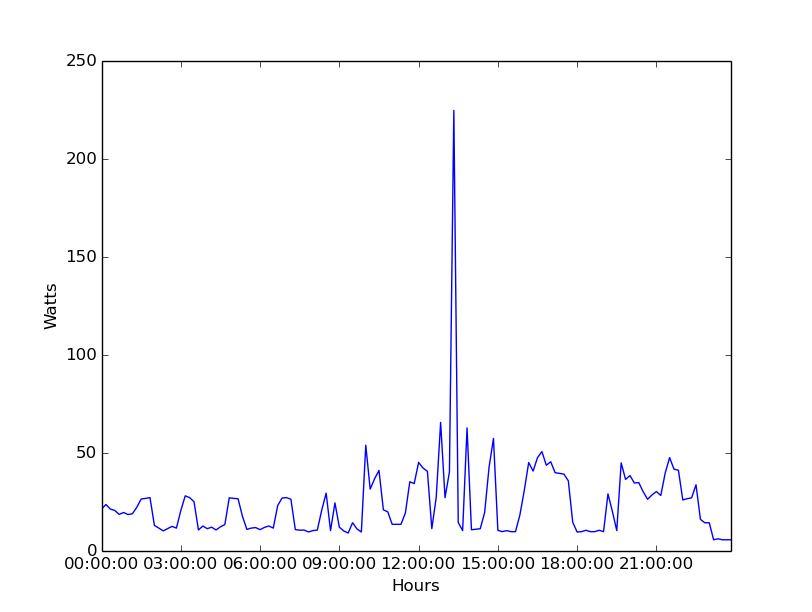
\includegraphics[width=1.0\textwidth]{img/only_interactive.png}
\caption[Difference]{\emph{\small Total consumption for interactive loads.}}
\label{interactiveLoads}
\end{figure}

\subsection{Results}
The total consumption trace of the household is illustrated in figure \ref{CompPlots}. The dashed blue line represents the original trace while the solid red line represents the trace with our scheduling algorithm least slack first (LSF). From the plot it is possible to see that the highest peak has been lowered from approximately 330 to 230 watts. Note that we already have a high peak in the interactive load. In the original trace without LSF, when both the fridge and the floor heater is powered  the peak is approximately 100 watts higher. With LSF on the other hand, the scheduler powers down both background loads at critical times. During the other hours the original and the LSF trace looks similar. There are just a few places where the solid line is significantly higher than the blue. This happens after the highest peak at 800 minutes. This happens since with LSF the execution of the background loads are postponed and will therefore yield in peaks later in time. These peaks however, never gets higher than the one caused by the interactive loads.

\begin{figure}[!ht]
\centering
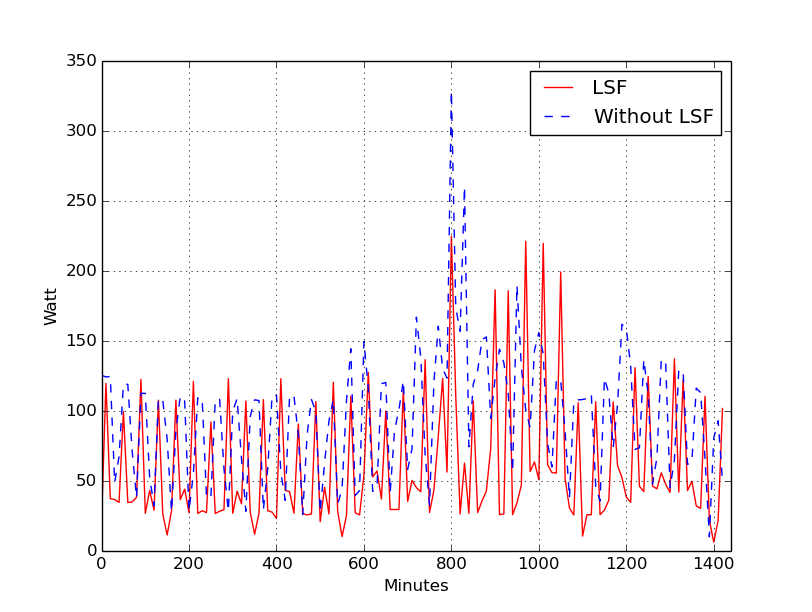
\includegraphics[width=1.0\textwidth]{img/comparizon.png}
\caption[Difference]{\emph{\small Power trace comparison during a 24-hour period.}}
\label{CompPlots}
\end{figure}

One of the issues with our test data is the large impact on the consumption caused by the floor heater. The floor heater frequently stands for more than 60 percent of the household's total consumption when active. This makes the consumption trace relatively pointed. Every time the floor heater is powered up, a spike in the consumption is noticed. A test set with more interactive loads and more background loads to control might help smoothing out the curve and yield in an even better consumption trace. Although it is wanted to avoid the worst peaks, a completely flat consumption is easier for the power suppliers to handle.

\subsection{Challenges}
\label{sec:challenges}
In this section we describe some of the challenges that we have faced. The challenges are related to the implementation of the system as well as the general idea itself.

\subsubsection{Third-party Library}
As we mentioned earlier we have used \emph{Plugwise} to implement this system. As there exists several other similar products we recommend using a product which has an open API. Since \emph{Plugwise} only offers a Windows based software with limited functions we had to program our own. We also wanted to prove that the solution easily can run on a Raspberry Pi, so we had to develop our own software for Debian/Linux operating system. Luckily, we found a third-party library for Python which we used \cite{hadaraplugwise}. The library turned out to have a couple of bugs which made it harder to use.

\subsubsection{Limitation of Test-data}
One of the biggest challenges is to find applicable test data. One or several real households need to be monitored with high granularity in order to observe how well the algorithm copes with sudden changes in the demand. Our test data is limited to one home during 24 hours and there are only a few devices that are being monitored. Furthermore, we only have the capability to control two background loads. Therefore, it is important to mention that the solution must be tested more thoroughly to evaluate the efficiency.

\subsubsection{The Threshold}
In order to have an efficient algorithm the threshold needs to be decided with great care. A threshold set too low will cause the scheduler to push the execution of the background loads on to the future, until the slack is zero and they are forced to run. This may lead to a forced execution in an inappropriate time. On the other hand, a threshold set too high would make the scheduler run all background loads simultaneously and then turn them all off when they reach their bound, yielding in a high peak followed by a low through.

\subsubsection{Infrastructure}
To get a system like this installed in a home today would require some effort. All background loads need to be equipped with smart plugs and sensors to be able to control and schedule them. Just to equip them with smart plugs is quite easy, but to equip them all with sensors as well is not as trivial. A better solution would be to use the already existing sensors in the appliances. This however, requires communication between the appliances and the scheduler. Even though more and more devices receive communication features, the so-called Internet of things, the vast majority of home appliances still cannot communicate.